Dans ce chapitre nous présentons un langage impératif permettant de modéliser C.
Nous donnons sa syntaxe ainsi qu'une sémantique opérationelle.

Ce langage servira de support aux systèmes de types décrits dans les
chapitres~\ref{cha:typbase}, \ref{cha:qualuser} et \ref{cha:qualsz}.

La traduction depuis C sera explicitée dans le chapitre~\ref{cha:implem}.

\section{Syntaxe}

\begin{figure}
\gramlr{Programmes}{
\begin{align*}
P \gramisa & (\vec{f}, \vec{v}, b) & \textrm{Fonctions, globales, initialiseur}
\end{align*}
}

\gramlr{Expressions}{
\begin{align*}
e  \gramisa & lv              & \textrm{Left-value}
\\ \gramor  & \textrm{op}~e   & \textrm{Opération unaire}
\\ \gramor  & e~\textrm{op}~e & \textrm{Opération binaire}
\\ \gramor  & cst             & \textrm{Constante}
\\ \gramor  & \& lv           & \textrm{Pointeur sur donnée}
\\ \gramor  & \& f            & \textrm{Pointeur sur fonction}
\end{align*}
}

\gramlr{Opérateurs}{
\begin{align*}
\textrm{op} \gramisa & +,-,\times,/         & \textrm{Arithmétique entière}
\\          \gramor  & +.,-.,\times.,/.     & \textrm{Arithmétique flottante}
\\          \gramor  & =,≠,≤,≥,<,>          & \textrm{Comparaisons}
\\          \gramor  & \&,|,\textasciitilde & \textrm{Opérateurs bit à bit}
\\          \gramor  & \&\&,||,!            & \textrm{Opérateurs logiques}
\\          \gramor  & ⋘, ⋙                 & \textrm{Décalages}
\end{align*}
}

\todo{XOR}

\gramlr{Left-values}{
\begin{align*}
lv \gramisa & var      & \textrm{Variable}
\\ \gramor  & lv.champ & \textrm{Accès à un champ}
\\ \gramor  & lv[e]    & \textrm{Accès à un tableau}
\\ \gramor  & *e       & \textrm{Déréférencement}
\end{align*}
}

\gramlr{Blocs}{
\begin{align*}
b  \gramisa & i ; b & \textrm{Séquence}
\\ \gramor  & ε     & \textrm{Bloc vide}
\end{align*}
}

\gramlr{Instructions}{
\begin{align*}
i  \gramisa & lv \leftarrow e             & \textrm{Affectation}
\\ \gramor  & lv \leftarrow funexp (args) & \textrm{Appel de fonction}
\\ \gramor  & funexp (args)               & \textrm{Appel de procédure}
\\ \gramor  & \npkDecl{nom}{b}            & \textrm{Déclaration}
\\ \gramor  & \npkIf{e}{b}{b}             & \textrm{Alternative}
\\ \gramor  & \npkDoWith{b}{label}        & \textrm{Nommage de bloc}
\\ \gramor  & \npkGoto{label}             & \textrm{Saut en avant}
\\ \gramor  & \npkWhile{b}                & \textrm{Boucle infinie}
\\ \gramor  & \npkReturn{e}               & \textrm{Retour de fonction}
\end{align*}
}

\todo{Fonctions}

\caption{Syntaxe d'un langage impératif}
\label{fig:syntx}
\end{figure}

\todo{Fonctions}

\todo{Ajouter l'arithmétique des pointeurs + types}

La figure~\ref{fig:syntx} définit un langage impératif. On suppose qu'on peut
compiler un programme écrit en C vers ce langage.

Un programme est un triplet $P = (\vec{f}, \vec{v}, b)$\footnote{ dans tout ce
chapitre on utilise la notation des vecteur pour les collections ordonnées :
$\vec{f} = (f_1, f_2, …, f_n)$, $\vec{v} = (v_1, v_2, …, v_p)$ (leur
cardinalités ne sont pas forcément égales).} constitué d'un ensemble de
fonctions, d'un ensemble de variables et d'un bloc d'instructions. Ce bloc sera
exécuté au lancement du programme ; il peut par exemple contenir le code
d'initialisation des variables globales et l'appel à la fonction principale.

\todo{expliquer pourquoi un while expr ne suffit pas}

Les différences principales avec C sont les suivantes :

\begin{itemize}
\item
  le flôt de contrôle est simplifié : les seules constructions sont
  l'alternative, la boucle infinie et le saut en avant.
\item
  les expressions sont sans effets de bords. En particulier, leur
  évaluation peut être faite sans modifier l'environnement.
\item
  les opérateurs pour entiers et les flottants sont différenciées.
\end{itemize}

\section{Sémantique}

Dans cette section, nous définissons une sémantique pour ce langage impératif ;
elle pourra servir à l'implantation d'un interpréteur et à raisonner de manière
formelle sur les programmes. Mathématiquement, cela consiste en la définition
d'une relation de transition $\rightarrow$ entre états de l'interpréteur.

Un état est constitué d'une part d'un point de contrôle dans le programme
(section~\ref{sec:cfg}, et d'autre part de l'état $σ$ de la mémoire
(section~\ref{sec:sigma}).

\subsection{État de l'interpréteur}

$Γ ⊢ (b, k, σ) → (b', k', σ')$

\[
\irule{Instr-Goto}
{(lbl, b') ∈ k}
{Γ ⊢ (\npkGoto{lbl} :: b, k, σ) → (b', k \backslash lbl, σ)}
\]

\[
\irule{Instr-DoWith}
{ }
{Γ ⊢ (\npkDoWith{b}{lbl} :: b', k, σ) → (b@b', k [lbl ↦ b'], σ)}
\]

\todo{not exactly for dowith}

\[
\irule{Instr-While}
{ }
{Γ ⊢ (\npkWhile{b} :: b', k, σ) → (b @ \npkWhile{b}, k, σ)}
\]

\todo{add b' at the end ?}

\begin{center}\rule{3in}{0.4pt}\end{center}

$Γ, k ⊢ (b, σ) → (b', σ')$

\[
\irule{Instr-Goto2}
{(lbl, b') ∈ k}
{Γ, k ⊢ (\npkGoto{lbl} :: b, σ) → (b', σ)}
\]


\[
\irule{Instr-DoWith2}
{Γ, k [lbl ↦ b'] ⊢ (b, σ) → ([], σ')}
{Γ, k ⊢ (\npkDoWith{b}{lbl} :: b', σ) → (b', σ')}
\]

\todo{doesn't work either, eg if inner block escapes}

\[
\irule{Instr-While2}
{ }
{Γ, k ⊢ (\npkWhile{b} :: b', σ) → (b @ \npkWhile{b}, σ)}
\]

\begin{center}\rule{3in}{0.4pt}\end{center}

Emprunté à Blazy et Appel\cite{cminorSL}

\gramlr{Continuations}{
\begin{align*}
k  \gramisa &  k_{pass}          & \textrm{Identité}
\\ \gramor  &  k_{seq}  (b,k)    & \textrm{Séquence}
\\ \gramor  &  k_{blk}  (lbl,k)  & \textrm{Nommage de bloc}
\\ \gramor  &  k_{goto} (lbl)    & \textrm{Saut}
\end{align*}
}

Relation :

$Γ ⊢ (k, σ) → (k', σ')$

Continuation initiale :

$k_0 ((\vec{f},\vec{v},b)) = k_{seq} (b, k_{pass})$

Règles d'évaluation :

\[
\irule{Instr-Goto3-direct}
{ }
{ Γ ⊢ ( k_{goto}  (lbl) . … . k_{blk} (lbl, k), σ) → (k, σ) }
\]

\[
\irule{Instr-Goto3-indirect}
{ lbl ≠ lbl' }
{ Γ ⊢ ( k_{goto} (lbl) . … . k_{blk} (lbl', k), σ) → (k_{goto} (lbl) . k, σ) }
\]

\[
\irule{Instr-DoWith3}
{ }
{ Γ ⊢ (\npkDoWith{b}{lbl} . k, σ) → ( b . k_{blk}(lbl, k)) }
\]

\[
\irule{Instr-While3}
{ }
{ Γ ⊢ (\npkWhile{b} . k, σ) → (b . \npkWhile{b} . k, σ) }
\]

\subsection{Graphe de flot de contrôle}
\label{sec:cfg}

\wip{}

Dans la syntaxe ci-dessus, on peut classifier les instructions en deux familles:
celles qui définissent le flot de contrôle (\npkIf{$\cdot$}{$\cdot$}{$\cdot$},
\npkDoWith{$\cdot$}{$\cdot$}, \npkGoto{$\cdot$}, \npkWhile{$\cdot$}) et celles
qui définissent le flot de données. Une première transformation va transformer
chaque fonction en son graphe de flot de contrôle, défini comme suit :

\begin{itemize}
\item
  les nœuds sont des points de contrôle, qui représentent par exemple
  l'adresse mémoire de l'instruction qui vient d'être exécutée.
\item
  les arêtes sont soit des instructions ``de données'' (affectation,
  appel de fonction, déclaration), soit des conditions (ie une
  expression).
\end{itemize}

\begin{minipage}{0.5\textwidth}
\begin{Verbatim}[commandchars=\\\{\}]
\PY{k+kt}{int} \PY{n+nf}{gcd}\PY{p}{(}\PY{k+kt}{int} \PY{n}{a}\PY{p}{,} \PY{k+kt}{int} \PY{n}{b}\PY{p}{)}
\PY{p}{\PYZob{}}
    \PY{k}{if} \PY{p}{(}\PY{n}{a} \PY{o}{=}\PY{o}{=} \PY{l+m+mi}{0}\PY{p}{)} \PY{p}{\PYZob{}}
        \PY{k}{return} \PY{n}{b}\PY{p}{;}
    \PY{p}{\PYZcb{}}
    \PY{k}{while} \PY{p}{(}\PY{n}{b} \PY{o}{!}\PY{o}{=} \PY{l+m+mi}{0}\PY{p}{)} \PY{p}{\PYZob{}}
        \PY{k}{if} \PY{p}{(}\PY{n}{a} \PY{o}{\PYZgt{}} \PY{n}{b}\PY{p}{)} \PY{p}{\PYZob{}}
            \PY{n}{a} \PY{o}{=} \PY{n}{a} \PY{o}{-} \PY{n}{b}\PY{p}{;}
        \PY{p}{\PYZcb{}} \PY{k}{else} \PY{p}{\PYZob{}}
            \PY{n}{b} \PY{o}{=} \PY{n}{b} \PY{o}{-} \PY{n}{a}\PY{p}{;}
        \PY{p}{\PYZcb{}}
    \PY{p}{\PYZcb{}}
\PY{p}{\PYZcb{}}
\end{Verbatim}

\end{minipage}
\begin{minipage}{0.5\textwidth}
\begin{Verbatim}[commandchars=\\\{\}]
\PY{n}{int32} \PY{n+nf}{gcd}\PY{p}{(}\PY{n}{int32} \PY{n}{a}\PY{p}{,} \PY{n}{int32} \PY{n}{b}\PY{p}{)} \PY{p}{\PYZob{}}
    \PY{k}{if} \PY{p}{(}\PY{n}{a} \PY{o}{=}\PY{o}{=} \PY{l+m+mi}{0}\PY{p}{)} \PY{p}{\PYZob{}}
      \PY{o}{!}\PY{k}{return} \PY{o}{=} \PY{n}{b\PYZus{}int32}\PY{p}{;}
      \PY{k}{goto} \PY{n}{lbl0}\PY{p}{;}
    \PY{p}{\PYZcb{}}
    \PY{k}{while} \PY{p}{(}\PY{l+m+mi}{1}\PY{p}{)} \PY{p}{\PYZob{}}
        \PY{k}{if} \PY{p}{(}\PY{n}{b} \PY{o}{=}\PY{o}{=} \PY{l+m+mi}{0}\PY{p}{)} \PY{p}{\PYZob{}}
            \PY{k}{goto} \PY{n}{lbl1}\PY{p}{;}
        \PY{p}{\PYZcb{}}
        \PY{k}{if} \PY{p}{(}\PY{n}{a} \PY{o}{\PYZgt{}} \PY{n}{b}\PY{p}{)} \PY{p}{\PYZob{}}
             \PY{n}{a} \PY{o}{=} \PY{n}{a} \PY{o}{-} \PY{n}{b}\PY{p}{;}
        \PY{p}{\PYZcb{}} \PY{k}{else} \PY{p}{\PYZob{}}
             \PY{n}{b} \PY{o}{=} \PY{n}{b} \PY{o}{-} \PY{n}{a}\PY{p}{;}
        \PY{p}{\PYZcb{}}
    \PY{p}{\PYZcb{}}
    \PY{n+nl}{lbl1:}
    \PY{n+nl}{lbl0:}
    \PY{p}{;}
\PY{p}{\PYZcb{}}
\end{Verbatim}

\end{minipage}

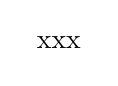
\begin{tikzpicture}
\node{xxx};
\end{tikzpicture}


Intuitivement, on peut "passer" d'un état à un autre soit en passant par une
arête "condition" qui s'évalue à une valeur "vrai", soit en appliquant les
effets de bord d'une arête "instruction".

Dans la suite, on suppose qu'on a à notre disposition un ensemble de jugements :
$\langle l, instr, l' \rangle$ qui signifie qu'on peut passer du point $l$ au
point $l'$ en effectuant l'instruction $instr$.

\subsection{État mémoire}
\label{sec:sigma}

L'interpréteur défini ici manipule des valeurs :

\gramlr{Valeurs}{
\begin{align*}
v  \gramisa  & n           & \textrm{Entier}
\\ \gramor   & f           & \textrm{Flottant}
\\ \gramor   & \cNil       & \textrm{Pointeur nul}
\\ \gramor   & \&a         & \textrm{Pointeur sur l'adresse $a$}
\\ \gramor   & \&f         & \textrm{Pointeur sur la fonction $f$}
\\ \gramor   & \top        & \textrm{Valeur non initialisée}
\end{align*}
}

On note l'ensemble des valeurs \textsc{Val}.

\begin{definition}[État mémoire]
L'interpréteur possède une mémoire, indexée par un ensemble d'adresses noté
\textsc{Addr}. Un état mémoire $σ$ est une fonction partielle de \textsc{Addr}
vers \textsc{Val}.
\end{definition}

\todo{Il faut une opération genre fromBytes}

\todo{Pile d'appels}

\begin{definition}[Fonction de transition]
La sémantique concrète que nous définissons ici est constituée de jugements
logiques. Le jugement principal est une relation de transition $\rightarrow$
entre états de l'interpréteur : il sera donc noté $Γ ⊢ (l, σ) \rightarrow (l', σ')$.
\end{definition}

\subsection{Jugements}

La sémantique concrète repose sur des jugements logiques et des règles
d'inférences, de la forme :

\[
\irule{Nom}{P_1 \\ … \\ P_n}{C}
\]

Les $P_i$ sont les prémisses, et $C$ la conclusion. Cette règle s'interprète de
la manière suivante : si les $P_i$ sont prouvées, alors $C$ est prouvée.

Certaines règles n'ont pas de prémisse : on parle alors d'axiome.

\[
\irule{Ax}{ }{A}
\]

Compte-tenu de la structure des règles, la preuve d'un jugement pourra donc être
vue sous la forme d'un arbre :

\[
  \irule{r1}{
    \irule{r2}
          {
            \irule{r3}
              { }
              {A_1}
              \\
            \irule{r4}
              { }
              {A_2}
          }
          {B_1}
    \\
    \irule{r5}
      {
        \irule{r6}
          { }
          {A_3}
        }{B_2}
      }{C}
\]

\subsection{Sémantique des left-values}

La mémoire est organisée en adresses, mais pourtant dans le programme cette
notion n'est pas directement visible. Les accès sont réalisés à travers des
"left values". Dans le langage C, elles correspondent aux constructions qui
peuvent se retrouver à gauche du signe "=" dans une affectation.

\begin{definition}[Correspondance left-values / adresses]
  Sous un environnement $Γ$ et un état mémoire $σ$, une left-value peut
  correspondre à une adresse $a$. Ceci sera noté $Γ, σ ⊢ lv ↝ a$.
\end{definition}

\begin{mathpar}
\irule{Eval-Lv-Var}{
  (v, a) ∈ σ
}{
  Γ, σ ⊢ v ↝ a
}
\and
\irule{Eval-Lv-Deref}{
  Γ, σ ⊢ e ⇒ \&a
}{
  Γ, σ ⊢ *e ↝ a
}
\and
\irule{Eval-Lv-Field}{
  Γ, σ ⊢ lv ↝ a
}{
  Γ, σ ⊢ lv.f ↝ a + f
}
\and
\irule{Eval-Lv-Array}{
  Γ, σ ⊢ lv ↝ a \\
  Γ, σ ⊢ e ⇒ n
}{
  Γ, σ ⊢ lv[e] ↝ a + n
}
\end{mathpar}

\subsection{Sémantique des expressions}

Les expressions sont les constructions syntaxiques de base du langage. Étant
donné un environnement et un état mémoire, on peut leur associer une valeur.

Par exemple, dans l'environnement qui à la variable $x$ associe l'adresse $a$ et
dans l'état mémoire qui à l'adresse $a$ associe la valeur $2$, l'expression $x +
3$ s'évalue en $5$.

\begin{definition}[Évaluation d'une expression]
  Sous un environnement $Γ$ et un état mémoire $σ$, une left-value peut
  produire une valeur $v$. Ceci sera noté $Γ, σ ⊢ e ⇒ v$.
\end{definition}

Dans le cas où l'expression est une constante, c'est directement le résultat.

\begin{mathpar}
\irule{Eval-Cst}{
}{
  Γ, σ ⊢ c ⇒ c
}
\end{mathpar}

Si l'expression est une left-value, on établit à quelle adresse elle correspond
et on récupère dans l'état mémoire à quelle valeur celle-ci correspond.

\begin{mathpar}
\irule{Eval-Lv}{
  Γ, σ ⊢ lv ↝ a \\
  (a, v) ∈ σ
}{
  Γ, σ ⊢ lv ⇒ v
}
\end{mathpar}

En ce qui concerne les opérations (unaires ou binaires), on commence par évaluer
les opérandes. Le résultat est l'opération "concrète" sur les valeurs, notée
$\widehat{\textrm{op}}$. Par exemple, pour la construction syntaxique $+$, on
utilise l'addition sur les valeurs $\widehat{+}$ (c'est-à-dire l'addition
usuelle).

\begin{mathpar}
\irule{Eval-Unop}{
  Γ, σ ⊢ e ⇒ v
}{
  Γ, σ ⊢ \textrm{op}~e ⇒ \widehat{\textrm{op}}~v
}
\and
\irule{Eval-Binop}{
  Γ, σ ⊢ e_1 ⇒ v_1 \\
  Γ, σ ⊢ e_2 ⇒ v_2
}{
  Γ, σ ⊢ e_1~\textrm{op}~e_2 ⇒ v_1~\widehat{\textrm{op}}~v_2
}
\end{mathpar}

Enfin, les adresses sont aussi des valeurs. Le cas des pointeurs sur fonction
est direct puisque toutes les fonctions sont globales ; pour le cas des
pointeurs sur données on commence par déterminer l'adresse de l'objet pointé
depuis l'état mémoire.

\begin{mathpar}
\irule{Eval-AddrOfFun}{
}{
  Γ, σ ⊢ \&f ⇒ \&f
}
\and
\irule{Eval-AddrOf}{
  Γ, σ ⊢ lv ↝ a
}{
  Γ, σ ⊢ \&lv ⇒ \&a
}
\end{mathpar}

\subsection{Sémantique des instructions}

La règle la plus simple concerne l'affectation : on peut affecter une
expressions à une left value si elles ont le même type.

\begin{mathpar}
  \irule{Instr-Assign}{
    \langle l, lv \leftarrow e, l' \rangle \\
    Γ, σ ⊢ lv ↝ a \\
    Γ, σ ⊢ e ⇒ v
  }{
    Γ ⊢ (l, σ) \rightarrow (l', σ [ a ↦ v ])
  }
\end{mathpar}

Déclarer une variable, c'est rendre accessible dans un bloc une variable non
initialisée, qui n'est plus accessible par la suite : Si on suppose qu'on peut
traverser le bloc interne $b$ sous un $σ$ enrichi d'une nouvelle variable $x$,
on peut donc traverser l'instruction \npkDecl{x}{b}.

\begin{minipage}{0.6\textwidth}
\begin{mathpar}
  \irule{Instr-Decl}{
    \langle l, \npkDecl{x}{b}, l' \rangle \\
    \langle l_b, b, l_b' \rangle \\
    σ' = σ ⊕ \{ x \rightarrow \top \} \\
    Γ ⊢ (l_b, σ', s) \rightarrow (l_b', σ'')
  }{
    Γ ⊢ (l, σ) \rightarrow (l', σ'' \backslash x)
  }
\end{mathpar}
\end{minipage}
\begin{minipage}{0.4\textwidth}
\begin{tikzpicture}
  [cfgnode/.style={draw,shape=circle},node distance=2cm]
  \node[cfgnode] (l) {$l$};
  \node[cfgnode,right of=l, node distance=4cm] (lp) {$l'$};
  \node[cfgnode,below of=l, xshift=1cm] (lb) {$l_b$};
  \node[cfgnode,below of=lp, xshift=-1cm] (lbp) {$l_b'$};
  \draw[->] (l)  to node[auto] {$↑x\{b\}$} (lp);
  \draw[->] (lb) to node[auto] {$b$} (lbp);
  \draw[->,dashed] (l) to node[auto] {$⊕ \{ x → \top \}$}(lb);
  \draw[->,dashed,swap] (lbp) to node[auto] {$\backslash x$} (lp);
\end{tikzpicture}

\end{minipage}

\todo{fcall}

TODO pour :

\[
\irule{Instr-Fcall}{
  \langle l, lv \leftarrow fe(\vec{e}), l' \rangle \\
  σ ⊢ fe ⇒ f \\
  Γ, σ ⊢ \vec{e} ⇒ \vec{v} \\
  σ' = σ ⊕ \{args(f) = \vec{v}\} ⊕ \{ !ret \rightarrow \top \} \\
  Γ ⊢ (Entry(f), σ') \rightarrow (Exit(f), σ'') \\
  Γ, σ'' ⊢ !ret ⇒ v_{ret} \\
  Γ, σ'' ⊢ lv ↝ a
}{
  Γ ⊢ (l, σ) \rightarrow (l', σ'' \backslash (args(f) \cup \{!ret\}) ⊕ \{ a \rightarrow v_{ret}\}, ?)
}
\]

\todo{definir $σ ⊢ fe ⇒ f$}

\subsection{Sémantique des conditions}

On utilise un encodage similaire à la déclaration. Tout d'abord, on évalue la
condition dans un contexte $σ$. Si elle s'évalue en un entier non nul, et qu'une
transition à travers le bloc $i_t$ est possible, alors on peut faire passer à
travers le "\textsc{If}".

\begin{minipage}{0.5\textwidth}
\begin{tikzpicture}
  [cfgnode/.style={draw,shape=circle}, node distance=1.5cm]
  \node[cfgnode] (l) {$l$};
  \node[cfgnode,right of=l, node distance=4.5cm] (lp) {$l'$};
  \node[cfgnode,below of=l, xshift=5mm] (lt) {$l_t$};
  \node[cfgnode,below of=lp, xshift=-5mm] (ltp) {$l_t'$};
  \node[cfgnode,above of=l, xshift=5mm] (lf) {$l_f$};
  \node[cfgnode,above of=lp, xshift=-5mm] (lfp) {$l_f'$};
  \draw[->] (l)  to node[auto] {$\npkIf{e}{i_t}{i_f}$} (lp);
  \draw[->] (lt) to node[auto] {$i_t$} (ltp);
  \draw[->] (lf) to node[auto] {$i_f$} (lfp);
  \draw[->,dashed] (l) to node [auto,swap] {$≠0$} (lt);
  \draw[->,dashed] (ltp) to (lp);
  \draw[->,dashed] (l) to node [auto] {$0$} (lf);
  \draw[->,dashed] (lfp) to (lp);
\end{tikzpicture}

\end{minipage}
\begin{minipage}{0.5\textwidth}
\begin{mathpar}
\irule{If-True}{
  \langle l, \npkIf{e}{i_t}{i_f}, l' \rangle \\
  Γ, σ ⊢ e ⇒ n \\
  n ≠ 0 \\
  \langle l_i, i_t, l_i' \rangle \\
  Γ ⊢ (l_i, σ) \rightarrow (l_i', σ')
}{
  Γ ⊢ (l, σ) \rightarrow (l', σ')
}
\and
\irule{If-False}{
  \langle l, \npkIf{e}{i_t}{i_f}, l' \rangle \\
  Γ, σ ⊢ e ⇒ 0 \\
  \langle l_i, i_f, l_i' \rangle \\
  Γ ⊢ (l_i, σ) \rightarrow (l_i', σ')
}{
  Γ ⊢ (l, σ) \rightarrow (l', σ')
}
\end{mathpar}
\end{minipage}
